\subsection{Composition does not pay once the hierarchy is in RAM}\label{sec:composition}

\begin{figure*}[tb]
\centering
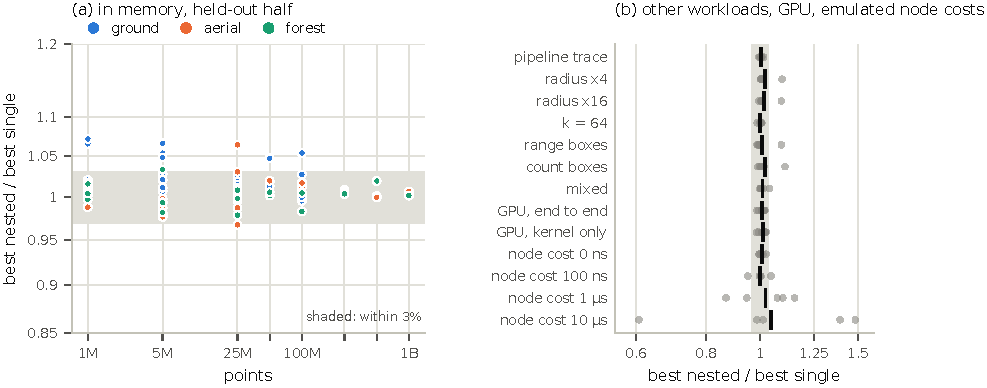
\includegraphics[width=\textwidth]{figures/fig_composition}
\caption{Best nested finalist over best single finalist. (a) The \nCells{} held-out cells against their size, coloured by scan group; the band marks the 3\% tie zone. (b) The same ratio on seven workload variants of six 100M clouds, on the GPU for the normal-estimation pass of six cells at two values of $k$, and under emulated per-node costs of 0 to 10\us{} on five 25M clouds; each dot is one cell and the bar its geometric mean.}
\label{fig:composition}
\end{figure*}

\begin{table*}[t]
\centering\footnotesize
\caption{Composition in memory, held-out and interleaved: the best nested finalist over the best single finalist per cell (geometric mean and range), wins, ties and losses at the 3\% band, the cells in which the confirmation step adopted a nested schema, and the pick over the fastest single timed on the test half.}
\label{tab:composition}
% generated by scripts/paper/tables.py; do not edit
\begin{tabular}{lrrrrrr}
\toprule
Cells & $n$ & nested picked & nested\,/\,single & range & wins\,/\,ties\,/\,losses & pick\,/\,oracle \\
\midrule
1M & 17 & 0 & 1.015 & 0.99--1.07 & 0\,/\,14\,/\,3 & 1.001 \\
5M & 16 & 0 & 1.013 & 0.98--1.07 & 0\,/\,11\,/\,5 & 1.002 \\
25M & 16 & 0 & 1.006 & 0.97--1.06 & 1\,/\,13\,/\,2 & 1.009 \\
50M & 6 & 0 & 1.017 & 1.00--1.05 & 0\,/\,5\,/\,1 & 1.000 \\
100M & 9 & 0 & 1.012 & 0.98--1.05 & 0\,/\,8\,/\,1 & 1.004 \\
250M & 3 & 0 & 1.006 & 1.00--1.01 & 0\,/\,3\,/\,0 & 1.001 \\
500M & 3 & 0 & 1.006 & 1.00--1.02 & 0\,/\,3\,/\,0 & 1.008 \\
1B & 3 & 0 & 1.004 & 1.00--1.01 & 0\,/\,3\,/\,0 & 1.000 \\
\midrule
ground & 31 & 0 & 1.020 & 0.98--1.07 & 0\,/\,24\,/\,7 & 1.004 \\
aerial & 25 & 0 & 1.005 & 0.97--1.06 & 1\,/\,21\,/\,3 & 1.004 \\
forest & 16 & 0 & 1.002 & 0.98--1.03 & 0\,/\,15\,/\,1 & 1.002 \\
\midrule
all & 73 & 0 & 1.011 & 0.97--1.07 & 1\,/\,60\,/\,12 & 1.003 \\
\bottomrule
\end{tabular}

\end{table*}

\begin{table}[t]
\centering\footnotesize
\caption{Composition in three other regimes: workload variants on the pipeline trace's centres (six 100M clouds), the GPU normal-estimation pass (six cells, $k = 16$ and $32$; fastest of three rotated rounds per schema), and an emulated cost added to every node a query enters (five 25M clouds, each cost with its own search). Below 1 the nested schema is faster.}
\label{tab:regimes}
% generated by scripts/paper/tables.py; do not edit
\begin{tabular}{lrrrr}
\toprule
Regime & $n$ & nested\,/\,single & range & picked \\
\midrule
workload base & 6 & 1.005 & 1.00--1.02 & -- \\
workload radius4 & 6 & 1.022 & 1.00--1.10 & -- \\
workload radius16 & 6 & 1.018 & 1.00--1.09 & -- \\
workload knn64 & 6 & 1.002 & 0.99--1.01 & -- \\
workload range8 & 6 & 1.010 & 0.99--1.09 & -- \\
workload count64 & 6 & 1.020 & 0.99--1.11 & -- \\
workload mixed & 6 & 1.011 & 1.00--1.04 & -- \\
\midrule
GPU, end to end & 12 & 1.010 & 0.99--1.02 & -- \\
GPU, kernel only & 12 & 1.013 & 0.99--1.03 & -- \\
\midrule
node cost 0 ns & 5 & 1.008 & 1.00--1.03 & 0 of 5 \\
node cost 100 ns & 5 & 1.000 & 0.95--1.05 & 1 of 5 \\
node cost 1 $\mu$s & 5 & 1.024 & 0.87--1.15 & 2 of 5 \\
node cost 10 $\mu$s & 5 & 1.046 & 0.61--1.48 & 1 of 5 \\
\bottomrule
\end{tabular}

\end{table}

\paragraph{In memory.} In none of the \nCells{} cells did the confirmation step adopt a nested schema (Table~\ref{tab:composition}). The best nested finalist is \nestedSingleAll$\times$ the best single over all cells, between \nestedSingleLo{} and \nestedSingleHi{} in any one cell: \nestedTiesAll{} ties, \nestedLossesAll{} losses and \nestedWinsAll{} win at the 3\% band. The ratio does not move with the size of the cloud (Figure~\ref{fig:composition}a): it is \nestedSingleHundredM{} at 100 million points and \nestedSingleOneB{} at one billion, where the transfer cells inherit a schema chosen at 250 million. It moves a little with the scan group: the ground scans lose the most to composition (\nestedSingleGround), the aerial surveys and the forests the least (\nestedSingleAerial{} and \nestedSingleForest). The pick, the schema the method would hand a user, is \pickOracleAll$\times$ the fastest single timed on the test half, so the selection itself works to within a fraction of a percent of an oracle; what it selects is a single, tuned structure.

Two things the nested finalists do win are build time and node count: they build about eight percent faster than the best single with about six percent fewer nodes, because the wide prefix replaces several binary levels. Neither buys query time, and the paper does not pursue them.

\paragraph{Other workloads.} The pipeline trace consists of small queries: a radius of a few centimetres, $k = 16$. Seven variants built on the same query centres of six 100M clouds (Table~\ref{tab:regimes}, Figure~\ref{fig:composition}b) ask for radii of four and sixteen times the trace's, $k = 64$, axis-aligned boxes of eight times the radius, counts over boxes of sixty-four times, and a mix of all of them. The best nested schema is between \workloadNestedSingleMin{} and \workloadNestedSingleMax$\times$ the best single on every variant, and the larger queries favour a leaf of 512 points for singles and nested schemas alike; on one cloud the nested schema loses nine to eleven percent on the large queries. No workload in the set gives composition a job.

\paragraph{On the GPU.} The same schemas were built into the same pool and queried by a warp-per-query kernel on an NVIDIA Quadro RTX 6000, for the normal-estimation pass of six cells (one $k$-nearest-neighbour query at every tenth point, $k = 16$ and $32$, ten million queries per run, with the normals computed in the kernel so that only normals and checksums leave the device). Each schema keeps its fastest of three rotated rounds, since the GPU was shared. The best nested schema is \gpuNestedSingleTotal$\times$ the best single end to end and \gpuNestedSingleKernel$\times$ in kernel time (\nGpuRows{} cell--$k$ pairs). The comparison that matters on the GPU is a different one: a specialised library, cudaKDTree~\cite{wald2022cudakdtree}, is \oursOverCudaKdTree$\times$ faster than the best of our schemas end to end, and no schema of ours, nested or single, closes that gap. Composition does not change the picture on the GPU; the implementation does.

\paragraph{Expensive nodes.} If a nested schema's fewer node visits are to pay, they should pay when a visit is expensive. A dial in the engine makes every query spin for a fixed time on each node it enters, in the search and in the held-out timing alike, so that each cost gets its own search, its own tuned singles and its own pick. From no added cost to 10\us{} per node on five 25M clouds, the best nested over the best single moves from \nodeCostNestedSingleZero{} to \nodeCostNestedSingleTenUs{} (Table~\ref{tab:regimes}): composition gets worse as nodes get dearer, not better. The confirmation step adopted a nested schema in a few cells at 1 and 10\us, and every one of those winners was matched or beaten by a single structure built from one of its own blocks at a larger leaf. What an expensive node calls for is a bigger leaf and a shallower tree, which cut the visits of a query from tens to a handful; a second primitive on top is a proxy for that and a worse one.

Section~\ref{sec:ooc} takes the last step and puts the nodes themselves on a storage device.
